%1234567890123456789012345678901234567890123456789012345678901234567890123456789
\chapter{Introduction}

The human desire of being physically impressive has a long history
dated back to ancient Greece.
The ancient Olympic Games celebrated the glory of physical dominance of
body strength, as well as athletic agility, to achieve the goals
faster and more effortlessly. 
Today, physical agility continues to captivate our imagination in
various areas, such as sports, entertainment, or robot industry.
In film or game industries, agile motions are important content to make
their games or movies more fun and entertaining.
Besides entertainment values, being agile and strong also holds great practical
values for robotic technologies,
which can help search and rescue.
When the Fukushima Daiichi nuclear meltdown occurred in 2011,
it was too dangerous for human operations because of high radiation levels.
A few robots were deployed to
measure temperature and radioactivity but failed due to limited speed and range
of operations \cite{Fukushima:2014:URL}.
The robots would have achieved the assigned tasks if they had
enough agility
%% to efficiently overcome disaster debris and locomote on uneven terrains. 
\revised{to locomote on uneven terrains and climb over disaster debris.}
%% \sehoon{Can ``overcome''=''jumping over debris''?}

Although ``agile'' motions include several examples, jumping,
vaulting, or rolling, they are not precisely defined to be discussed.
The word ``agile'' is defined as 
``able to move quickly, easily, effortlessly, and gracefully''.
While moving ``quickly'' can be directly associated with high-momentum
motions, moving ``easily'', ``effortlessly'', and ``gracefully'' are more
%% difficult to attach a physical meaning. \sehoon{Check English. Adding ``to''?}
%% \revised{difficult to define in physical terms.}
\revised{difficult to physically quantify.}
For instance, moving ``easily'' can be due to different reasons, such as the
innate strength of the subject, the accumulated 
experience, or the ability to negotiate with the environment.
In this disseration, we define ``agile motions'' as 
``able to move quickly and effortlessly in a complex environment''
, which highlights \revised{high momentum}
and well-coordinated strategies that exploit the environment.
One great example that showcases a suite of agile motions is Parkour,
a sport that features moving from the current location to the destination in
the most efficient way.
The skills of Parkour are well aligned with our definition of agile motions
because they require high momentum and dynamic planning to negotiate with the
obstacles and features in the environment.

The aim of this dissertation is to design a set of computational tools to
develop agile motor skills on virtual and real humanoids.
Although the grand goal would be to achieve agile motor skills on humanoid
robots, there are many unsolved practical issues to directly
design agile motions on the hardware,
such as \revised{control delays, sensor noises,} or safety concerns.
Unlike biped walking where adequate models and control theories are
already available, agile motions have not been studied extensively in the
literature of computer animation and robotics.
Therefore, the appropriate approach toward agile real humanoids is to first
develop theoretical models and control algorithms on the physics-based
simulation, where researchers in computer graphics can
%% accomplish complex and stunning tasks,
\revised{generate complex and impressive motions;}
\revised{then the next step is to} transfer the solution to real hardware
%% with the careful adjustment.
\revised{with additional processes, such as tuning parameters
  or revising control mechanisms.}
Simulation-developed solutions will
greatly reduce the expensive cost of hardware experiments and prevent
unexpected dangerous situations.

Agile motor skills are difficult tasks for humanoids.
General characteristics of agile motions, high momentum or frequent changes
of contacts, increase difficulties of most existing issues in motor control
problems tremendously
by requiring accurate control routines and efficient planning algorithms.
In addition to the existing issues, agile motions generate few more unique
challenges that need to be addressed. 
% First: falling and landing motions
The first issue is to ensure the safety of humanoids.
Because learning and executing agile motions often accompany both intentional
and inadvertent falls, it is necessary to learn how to fall safely without
introducing large damage.
% Second: general learning
Secondly, agile motions are not \revised{well-understood} unlike other motions,
such as running or reaching.
They cover a wide range of diverse skills, such as jumping, vaulting, or
rolling which are governed by different control mechanisms and principles.
We want to develop a set of general computational tools for \revised{designing}
a variety of agile motion controllers, instead of manually designing all
controllers individually.  
% Third: export
Finally, simple agile motion trajectories that are developed in virtual
simulation are less likely to work on physical systems
because small errors can be quickly accumulated and result in drastic deviations
from the original agile motions.
The discrepancy between virtual and real systems must be handled
systematically for utilizing simulation-optimized solutions.
% Therefore..
These additional, unique challenges motivated us to address the following 
problems in this dissertation, as steps to achieve agile motions 
on virtual and real humanoids.

\section{Falling Strategies for Humanoids}
% Introduction on the falling - Motivation, Description, Goal
Falling and landing motions are a set of fundamental motor skills
in various agile motions to protect humanoids themselves.
Because athletic movements frequently involves
transitions between airborne and contact phases, \revised{humanoids} must know
how to absorb the shock at the landing moment and avoid damage to the body
parts. 
In addition, well-executed falling motions will lead a smooth transition to the
next \revised{motion}.
%% %% Version 1.0
%% In this dissertation, we will discuss two different falling scenarios, 
%% of virtual and real humanoids.
%% For a virtual humanoid, we will describe a physics-based controller that allows
%% the character to fall from a wide range of heights and initial speed, 
%% which are inspired by agile falling and landing of Parkour practitioners.
%% For a real humanoid, we will propose a falling strategy for managing unexpected
%% falls due to a wide range of perturbations.

%% %% Version 1.1
%% \revised{In this dissertation, we will describe two different falling
%%   controllers for virtual and real humanoids.
%%   For a virtual humanoid, the entire falling sequence from the airborne, 
%%   the impact, and the rolling phases is discussed, which is inspired by agile
%%   falls of Parkour practitioners.
%%   For a real humanoid, we focused on falls on the ground, which are initiated
%%   by unexpected perturbations.
%%   In both scenarios, our falling controllers are able to handle a wide range of
%%   initial conditions, including heights and initial speeds.}
%% Version 1.2
\revised{In Chapter 3 and 4, we describe two different falling
  controllers for virtual and real humanoids.
  For a virtual humanoid, we discuss falls with the airborne phases, which are
  inspired agile jumping and falling motions of Parkour practitioners.
  On the other hand, we focused on falls without the airborne phases for real
  humanoids, which can be initiated by unexpected perturbations.
  In both scenarios, our falling controllers are robust enough to handle a wide
  range of initial conditions, such as heights and speeds.}
The effectiveness of both presented strategies are validated by measuring
amounts of joint stresses or contact forces to body parts in physics
simulation, and experimentally tested on a small-size humanoid.

\subsection{Falling and Landing Motion Control for Virtual Characters}
% Goal, Method (Strength), Verification + Image

In Chapter 3, we show how to create a robust controller for generating 
agile and natural falling motions of the virtual character that can land from 
various heights and velocities.
The goals of the controller are to reduce the joint stress at the impact and
get back on its feet to prepare the next action (\figref{intro_landing}).

\begin{wrapfigure}{r}{0.5\textwidth}
 \vspace{-25pt}
  \begin{center}
    %% 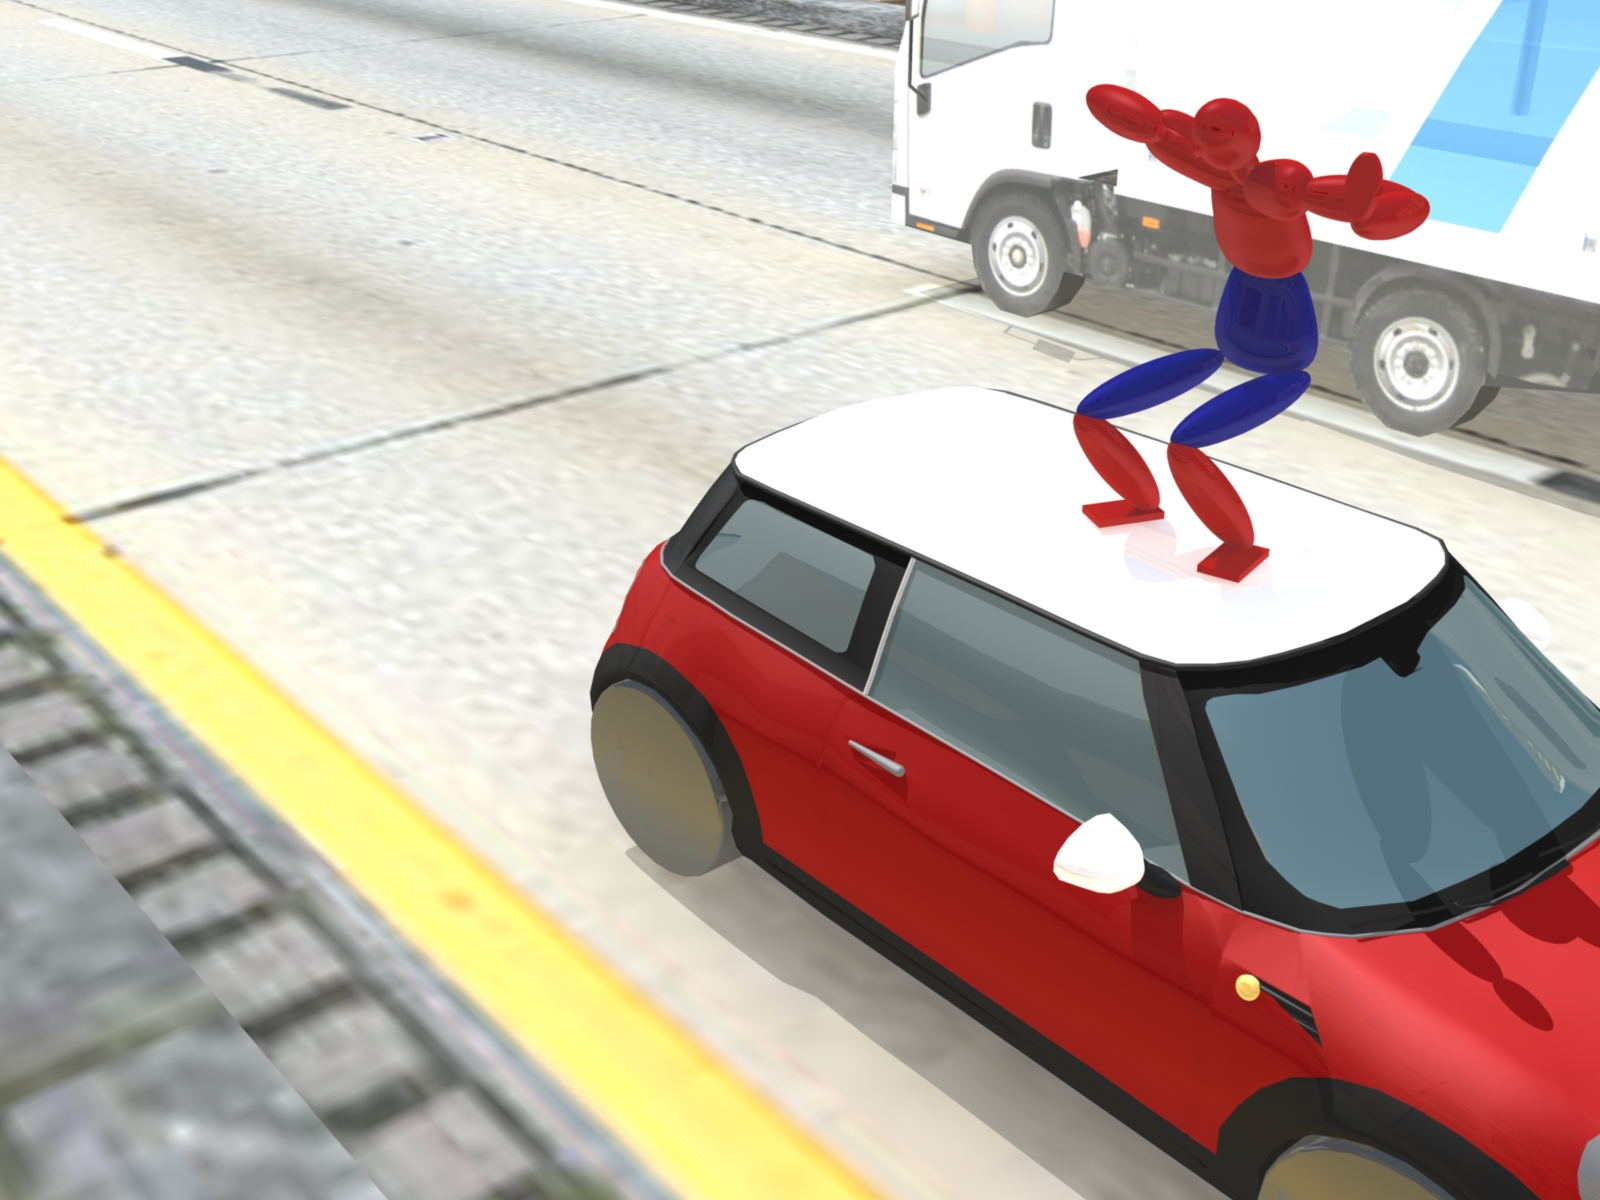
\includegraphics[width=0.48\textwidth]{images/intro_landing.jpg}
    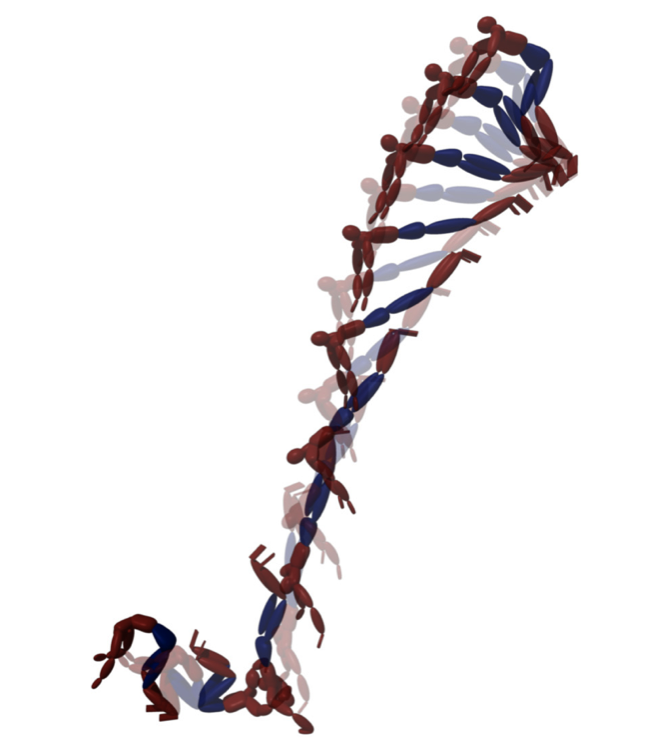
\includegraphics[width=0.48\textwidth]{images/intro_falling_sequence.png}
  \end{center}
   \vspace{-25pt}
  \caption{A fall of a virtual character.}
  \label{fig:intro_landing}
   \vspace{-10pt}
\end{wrapfigure}

Inspired by falling skills of Parkour, 
we formulate the falling problem
with three phases, \emph{airborne}, \emph{impact}, and \emph{rolling}
based on the contact states of a virtual character.
First, two sub-controllers are designed for the \emph{airborne} and
\emph{rolling} phases and a regression analysis is conducted to find 
an optimal landing angle that can connect two sub controllers at the
\emph{impact} phase.
we will demonstrate that the motion generated by the proposed controller
looks natural and induces smaller joint stress, which is still four times lower
than a uncontrolled rag-doll motion.


\subsection{Multiple Contact Planning for Humanoid falls}
\begin{figure}[h]
 %% \vspace{-25pt}
  \begin{center}
    %% 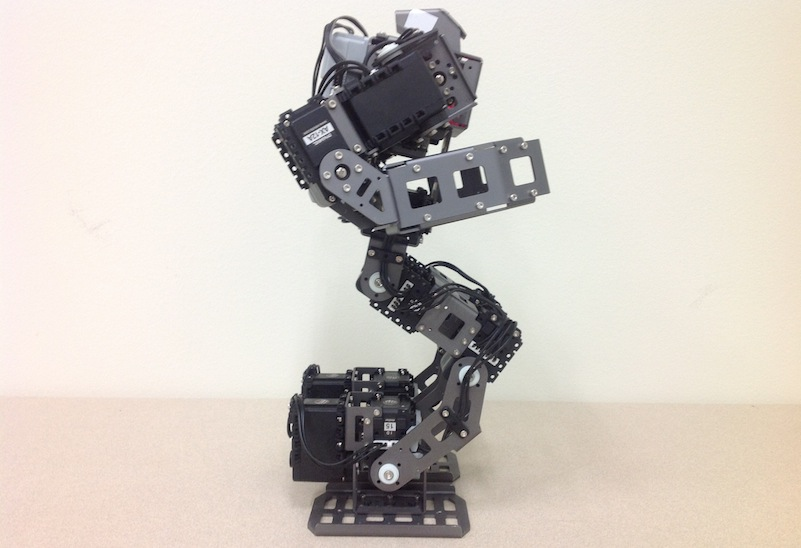
\includegraphics[width=0.48\textwidth]{images/intro_hardware.jpg}
    
\includegraphics[width=1.0\textwidth]{images/intro_gp_tripod}
  \end{center}
   %% \vspace{-25pt}
  \caption{A two-step falling strategy of a humanoid robot}
   %% \vspace{-10pt}
  \label{fig:intro_hardware}
\end{figure}
% Goal, Method (Strength), Verification + Image
Chapter 4 describes a robust falling strategy which plans for appropriate 
responses to a wide variety of falls, from a single step to recover
\revised{from} a gentle nudge, to a rolling motion to break a high-speed fall.
Our key observation is that many existing falling techniques
\cite{Wang:2012:WTO,Yun:2014:TFC,ZenpoUkemi:2014:URL}
assume specific sequences of contacts and aim to break specific ranges of
falls and requires us to an additional decision layer to choose the best
falling strategy to the given state.
Instead, our multiple contact planning algorithm provides a unified framework
for various existing falling strategies, which can adjust the number and order
of \revised{contacts} with respect to different magnitudes of perturbations.
In the proposed continuous space of strategies, our algorithm can efficiently
find the best \revised{contact sequences} for the given initial state using a
simplified model and dynamic programming.
To verify our framework, a variety of scenarios are tested on simulated
humanoids and the actual hardware (\figref{intro_hardware}) to show that our
algorithm plans versatile \revised{and effective} falling strategies
\revised{that successfully reduce damage to robots.}
%% with different contact sequences. 

\section{Learning Framework for General Agile Motions}
% Introduction on the learning - Motivation, Description, Goal
Unlikely well-defined tasks such as reaching or walking,
agile motions cover a wide range of diverse skills such as vaulting, flipping,
or rolling.
Because these agile motions are governed by different mechanisms and
principles, manually designing and fine-tuning specialized controllers for all
tasks is not a practical approach.
Design of an individual physics-based controller for a new motor skill is 
a time-consuming task which requires a lot of manual efforts from the controller
designer, from the design of the control mechanism to the tweaking of low-level
control parameters. 
%% %% Version 1.0
%% To simplify the costly learning process, we will introduce an intuitive and 
%% interactive framework for developing controllers that is inspired by
%% how humans learn dynamic motor skills through a iterative process of coaching
%% and practicing.
%% %% Version 1.1
%% \revised{We propose a novel framework to expedite
%%   the design process of controllers for general agile motions.
%%   The important component of the learning framework is an intuitive interface,
%%   which must be easy to use and general enough to train a variety of agile
%%   motor skills, including jumps, flips, vaults, and rolls.
%%   Further, the parameters of designed controllers must be efficiently optimized
%%   to reduced turn-around time.}
%% Another important component for the iterative controller design process
%% is an efficient optimization \revised{of control parameters} to reduce a
%% turn-around time. 
%% %% Version 1.2
%% \revised{We propose a novel framework to expedite
%%   the design process of controllers for general agile motions.
%%   Our learning framework allows users to intuitively and interactively }

%% Version 1.3
\revised{Our goal is to design intuitive and efficient learning framework for
  general motor skills, including jumping, flipping, vaulting, and rolling.
  %% The intuitiveness of the framework is achieved by proposing a novel interactive
  %% interface that designs controllers only using human-readable instructions, which
  %% are inspired by how humans teach dynamic motor skills.
  For an easy-to-use learning framework,
  we develop a nover interactive interface that designs controllers only using
  human-readable instructions inspired by how human coaches teach dynamic motor
  skills. 
  Further, the parameters of the designed controllers are efficiently optimized
  using our novel algorithms to reduce a turn-around time.
  Using the proposed interface and optimization techniques,
  users can intuitively and easily develop controllers for general agile motor
  skils on virtual characters. }

%% In this purpose, we propose two optimization techniques that can extend the
%% popular policy search algorithm, CMA-ES, to accelerate the convergence rate
%% and to optimize a parametrized objective function.

\subsection{Iterative Design of Dynamic Controllers}
% Goal, Method (Strength), Verification + Image
\begin{figure}[h]
 %% \vspace{-25pt}
  \begin{center}
    %% 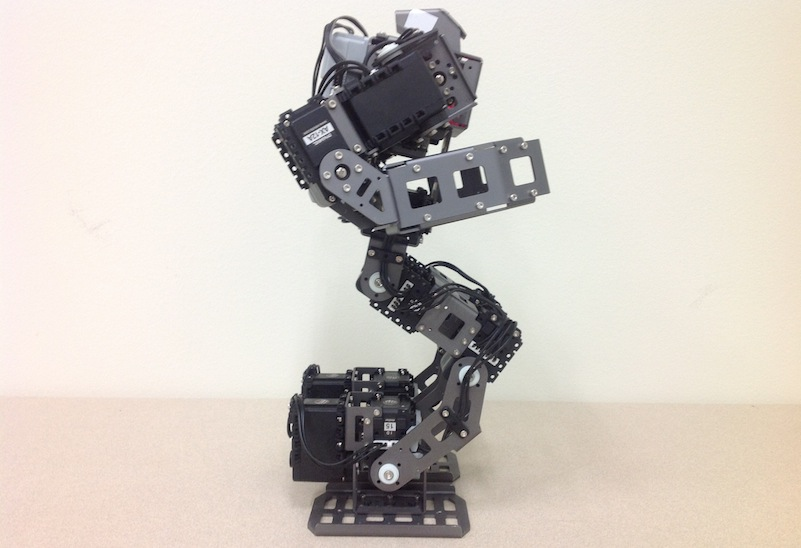
\includegraphics[width=0.48\textwidth]{images/intro_hardware.jpg}
    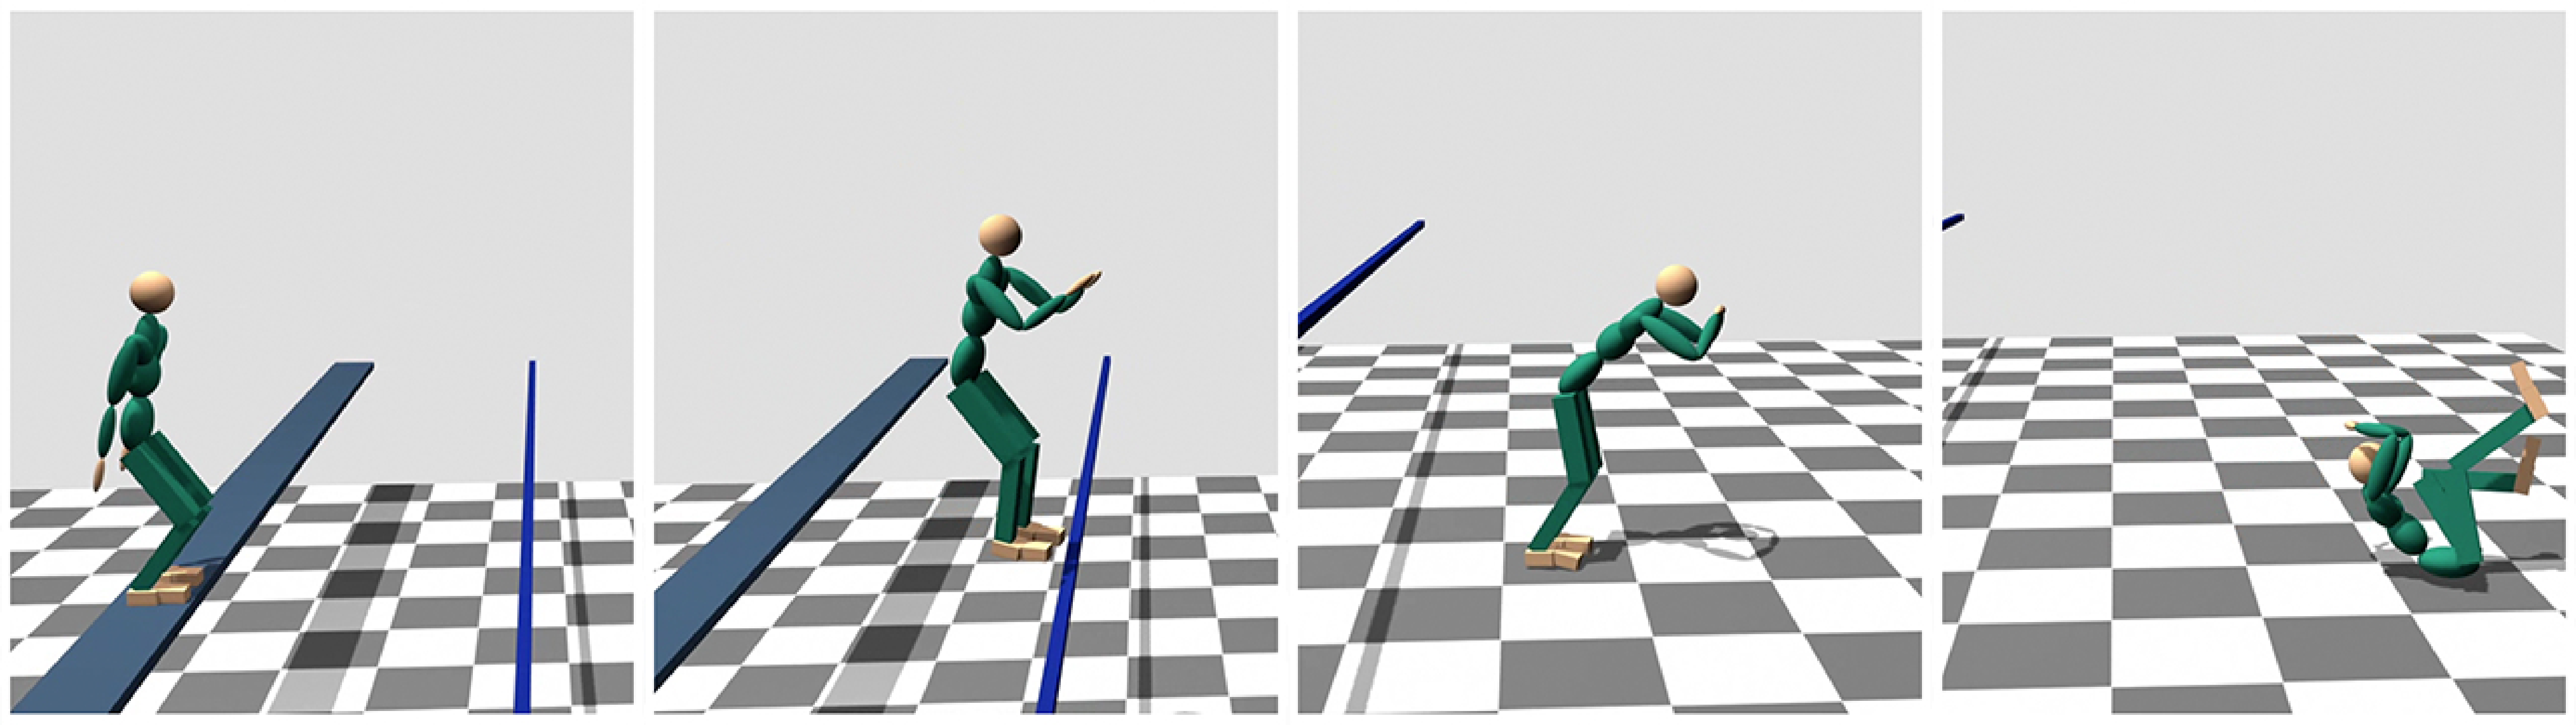
\includegraphics[width=1.0\textwidth]{images/intro_drop_roll}
  \end{center}
   %% \vspace{-25pt}
  \caption{A challenging stunt that a character jumps twice and rolls
    on the ground.}
   %% \vspace{-10pt}
  \label{fig:intro_drop_roll}
\end{figure}
%% \begin{wrapfigure}{r}{0.6\textwidth}
%%  \vspace{-10pt}
%%   \begin{center}
%%     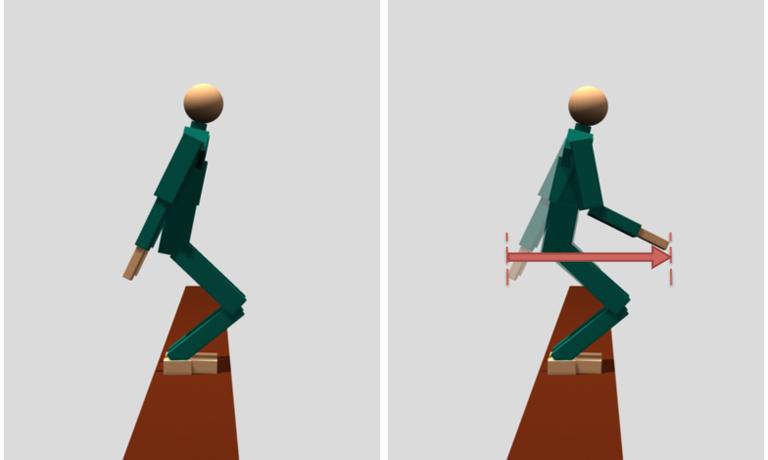
\includegraphics[width=0.58\textwidth]{images/intro_teach.png}
%%   \end{center}
%%    \vspace{-25pt}
%%   \caption{The proposed learning frame uses human readable instructions
%%     to teach motions.}
%%   \label{fig:intro_teach}
%%    \vspace{-10pt}
%% \end{wrapfigure}

In Chapter 5, we describe an iterative framework to design physics-based
controllers that executes very agile stunts (\figref{intro_drop_roll}).
The aim of this chapter is to design an intuitive and interactive framework
that a user can easily design complex controllers only using high-level,
human-readable instructions, 
which is inspired by a human learning process of coaching and practicing stages.
%% \sehoon{In the coaching stage, a user can 1) what to do 2) what not to do, constraints.}
\revised{During the coaching stage, the user provides instructions to revise
  the task objective, add constraints, or update control mechanisms based on
  the current skill level.}
To enable interactive coaching, we introduce ``control rigs'' as
an intermediate layer of control module which allows more coordinated control
of the low level control variables and and provides more intuitive mapping to
high-level human instructions. 
During the practicing stage, control parameters are efficiently determined
using CMA-ES, which will be further improved in the following chapters.
The details of controllers development process using our iterative learning
framework are shown with example iterative training procedures of Parkour
motions.

\subsection{Optimization with Failure Learning}
% Goal, Method (Strength), Verification + Image
In Chapter 6, we describe a new optimization algorithm for
\revised{highly constrained problems, which happens when the user imposes a
  lot of instructions to the virtual character.}
A controller with many constraints is difficult to be optimized due to the
relatively small feasible regions with many local minima.
Our key idea comes from human’s ability to learn from failure. 
Because failure in the real world is usually associated with pain or injury,
humans tend to be very effective in characterizing the cause of failure and
trying to avoid the same mistakes in the future. 
Under the concept of ``learning from failure'', \revised{the} proposed algorithm CMA-C
(Covariance Matrix Adaptation with Classification) utilizes the failed
simulation trials to approximate an infeasible region in the space of control
rig parameters so that it can predict validity of newly generated samples,
resulting \revised{in} a faster convergence than the standard CMA-ES.

\subsection{Optimization for Parametrized Motor Skills}
% Goal, Method (Strength), Verification + Image
In Chapter 7, we explain an evolutionary optimization algorithm for
learning parameterized skills to achieve whole-body dynamic tasks.
The parametrization of the learned motor skills is an essential ability
because a robot can \revised{adapt} the skill to a new situation, without
learning the entire motor skill from scratch.
Instead of maintaining a single Gaussian distribution, 
the algorithm reduces the number of samples by evolving a parametrized
probability distribution which describes a mapping from a task parameter
to the optimal control parameters.
we test the proposed optimization algorithm for learning three parametrized
dynamic motor skills on a simulated humanoid robot, including jumping,
kicking, and walking. 

%% \section{Model-based Learning for Virtual and Real Characters}
\section{Transferring Controllers from Simulation to Hardware}
% Goal, Method (Strength), Verification + Images

\begin{wrapfigure}{l}{0.5\textwidth}
 \vspace{-10pt}
  \begin{center}
    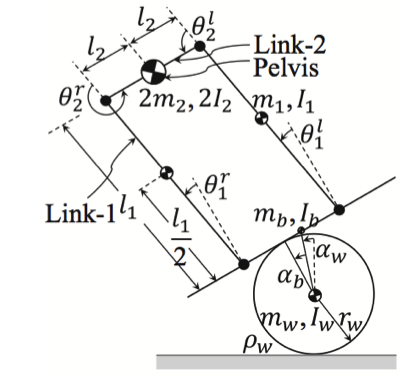
\includegraphics[width=0.35\textwidth]{images/intro_simple_robot.png}
  \end{center}
   \vspace{-25pt}
  \caption{A design of a simple legged robot on a bongoboard.}
  \label{fig:intro_bongo}
   \vspace{-10pt}
\end{wrapfigure}
In Chapter 8, we describe an iterative approach for learning 
hardware models and optimizing control policies using simulation.
The proposed learning framework is designed for reducing the number of
expensive hardware experiments. 
Computer simulation is often used to replace hardware experiments,
but it is difficult to obtain accurate simulation models and
simulation-optimized control policies are not likely to work on hardware.
To fill the gap between two system, we propose an algorithm for learning
hardware models and optimizing policies. 
Instead of learning hardware models from scratch, the proposed approach only
learns the difference from simulation models using Gaussian process.
As a proof of concept, we validate the algorithm on two different 
simulation models, one with perfect contacts and one with realistic contacts,
by finding a balancing controller for a simple bipedal robot on a bongo board
(\figref{intro_bongo}).

\section{Contributions}
The control and optimization methods discussed in this dissertation provide
several contributions to the computer animation and robotics community. 
These contributions are as follows:

\begin{itemize}
\item \textbf{A falling and landing strategy for virtual characters.}
  The falling strategy presented in the dissertation generates a natural falling
  and landing motion that falls from a wide range of heights and initial
  speeds, continuously rolls on the ground, and gets back on its feet without
  inducing large stress on joints at any moment.
\item \textbf{A multiple contact falling strategy for robots.}
  We introduce a falling strategy for humanoid robots
  to break a fall with minimal damage to the body parts
  by utilizing multiple contact points.
\item \textbf{An iterative learning framework for dynamic motor skills.}
  We propose an iterative and interactive learning framework 
  using human readable instructions that can teach a variety of agile motions
  to virtual characters.
  Starting from a basic controller, the proposed framework allows a user 
  to easily train complex physics-based controllers 
  with only intuitive high-level instructions from the user.
\item \textbf{An optimization technique for highly constrained problems.}
  We introduce a novel efficient optimization algorithm, CMA-C, that is 
  designed for the problem with many constraints and smaller feasible regions.
  The algorithm converges faster than the standard CMA-ES,
  by approximating the infeasible region using learned classifiers.
\item \textbf{An optimization technique for parametrized tasks.}
  We introduce an efficient evolutionary optimization algorithm for learning
  parametrized whole-body dynamic tasks.
  By evolving parameterized sample distributions, our algorithm
  converges faster than the baseline algorithm, CMA-ES.
\item \textbf{A model-based policy search for reducing hardware experiments.}
  We propose an iterative approach for learning hardware model and optimizing
  policies with as few hardware experiments as possible by learning
  \emph{dynamics bias}, which is difference between simulation and hardware
  models. 
\end{itemize}

%% \rule{0.95\textwidth}{1pt}

%% In the next chapter, we will discuss the related work conducted by other
%% researchers to address similar problems.

